\documentclass[11pt]{ECEtemp}

%%%%This is where you change your Name.Assignment.Class.etc...
\newcommand{\assignment}{Centered, Bold – 14 pt.:  Title of Report or Assignment}
\newcommand{\subdate}{April 29, 2019}
\newcommand{\class}{EE-2063  -  Microprocessors}
\newcommand{\Name}{Your Name, left justified, 11 or 12 pt. type}
\newcommand{\prof}{Dr. Nathan Hutchins}

\lstset{language=c}

\begin{document}
%%%Set up of the Name Section
\noindent
\Name \\ \class \\ \prof \\ \subdate 
%%%This places your title
\eceTitle{\assignment}
%%%Here is your report start! Good Luck!

\eceSection{Objective, Heading 1, Black lettering}
Describe the objective of the assignment or report. This includes the purpose of the report and a brief description of the results to be reported. For example: This template provides guidance on formatting and organizing a laboratory or design report to make the report more readable and more informative, and to abide more closely with the standard reporting formats of industry.

\eceSection{Introduction, (for design reports)}
Describe in a paragraph or two what you are doing and why you are doing it, to give the reader enough background to understand what they are about to read.  For example:

An important aspect of an engineer’s job consists of effectively communicating the results of experiments, simulations, and/or theoretical investigations to their peers, management, and potential or current business partners and collaborators. Engineer’s skilled in effective communication are more valued by their company or organization in general. This report describes a general method for organizing and presenting information that will enhance the user’s ability to effectively communicate their work.

\eceSection{Equipment or Tools Used}
\begin{itemize}
\itemsep0em %Reduce the space between items of the list!
\item   Equipment name and make (e.g. Agilent Oscilloscope, model \#xxxxx)
\item   MATLAB with Simulink
\item   Circuit Lab
\end{itemize}

\eceSection{Methodology}
\noindent 1. Design requirements (design report) or Specific Objectives (lab report)
\begin{enumerate}[(a)]
    \itemsep0em %Reduce the space between items of the list!
    \item Create a design report that is well-organized, comprehensive, and easy to read
    \item Determine the relationship between Thevenin voltage, Norton current, and Thevenin resistance
\end{enumerate}

\noindent 2. Description of Design Process (design report) or Sequence of Measurement/Analysis (lab report)

In this section, describe in a logical order how you proceeded in designing, analyzing, and/or measuring the project element or element(s). This section can consist of word descriptions, tables, equations and figures.
\underline{}{For word descriptions:} Use paragraph form, proper syntax, proper punctuation, and complete sentences. Be as specific as possible – avoid frequent use of pronouns like it, its, their, and other pronouns that can cause confusion when reading. Define any acronyms that you use before using them in the rest of the report. For example, this report will discuss the signal-to-noise ratio (SNR) at several points, and the SNR will be important in communications class. All tables, equations, and figures must be referenced within the text of the word descriptions. Equations should be referred to by number, i.e. the formula for the time constant of the circuit is given in Equation (1) – also acceptable is saying the formula is given in (1). Figures should be referred to as Fig. \# -- for example, Fig. 2 shows the basic circuit configuration used. Tables should be referred to by name – for example, the different design choices are shown in Table 2.
Both in the text and in tables, numbers must be correctly reported and formatted. All numbers should use either Engineering Notation unless Scientific Notation is the accepted standard. For example, you should not report a current as 0.0000562 A, instead you should report it as 56.2 $\mu$A, or $56.2*10^{-6}$ A for Engineering Notation, and $5.62*10^{-5}$ or $5.62E-5$ for Scientific Notation. Similarly, use 20 k$\Omega$ or $20*10^3$ $\Omega$, not 20,000 $\Omega$. When performing calculations, especially with numbers obtained from measurements with a limited number of significant digits, you must maintain the correct number of significant digits throughout your calculations and in your final answers. If the multimeter has only 2 significant digits for voltage, and your measurement of resistance is accurate to 2 or 3 significant digits, the current calculated from these numbers should not contain 5 significant digits. For example, the reading from a multimeter is 2.54 V, and the resistance is measured as 1.54 k$\Omega$, the answer should be 1.65 mA, not 0.001649351 or 1.6493 mA, as this implies the original measurements contained 4 digit accuracy or more. All quantities and values used must contain units.
The use of special characters, superscripts, and subscripts is expected. You should not write microseconds as ``us'', you must use ``$\mu$s'' for example. Use $\Omega$ for resistance (don’t write out ``ohms,'' and ``kohms'' is not acceptable) and lower case omega ($\omega$) for radial frequency as other examples. Use x2 in text, not x2. Use R2 in text, not R2. For scientific notation, either use 4.25E2 or, preferably $4.25*10^2$.

\begin{enumerate}[(a)]
    \itemsep0em %Reduce the space between items of the list!
    \item where did you start? 
    \item what assumptions did you make, if any? 
    \item if you picked values instead of solving for them, tell the reader you did this, why you did this, and give a reason for the values you picked, 
    \item show calculations or analysis you performed to come up with other values you had to design (amplifier gain, resistor values, filter parameters, digital logic, etc.), and 
    \item  provide a completed design that you plan to test in the experimental part.
\end{enumerate}

For a lab report, you want to provide information such as
\begin{enumerate}[(a)]
\item What measurements did you make, and why?
\item How did you construct the circuit/system/simulation?
\item What equipment/software was used?
\end{enumerate}

\noindent
Formatting for this section is as follows:

\noindent
Formatting is numbered list, without the indent

\noindent
1. Design requirements (design report) or Specific Objectives (lab report)

\begin{enumerate}[(a)]
\item   Create a design report that is well-organized, comprehensive, and easy to read
\item   Determine the relationship between Thevenin voltage, Norton current, and Thevenin resistance
\end{enumerate}

\noindent
2. Description of Design Process (design report) or Sequence of Measurement/Analysis (lab report)
In this section, describe in a logical order how you proceeded in designing, analyzing, and/or measuring the project element or element(s). This section can consist of word descriptions, tables, equations and figures. 

\underline{For word descriptions:}  Use paragraph form, proper syntax, proper punctuation, and complete sentences.  Be as specific as possible – avoid frequent use of pronouns like it, its, their, and other pronouns that can cause confusion when reading. Define any acronyms that you use before using them in the rest of the report. For example, this report will discuss the signal-to-noise ratio (SNR) at several points, and the SNR will be important in communications class. All tables, equations, and figures must be referenced within the text of the word descriptions.  Equations should be referred to by number, i.e. the formula for the time constant of the circuit is given in Equation (1) – also acceptable is saying the formula is given in (1). Figures should be referred to as Fig. \# -- for example, Fig. 2 shows the basic circuit configuration used. Tables should be referred to by name – for example, the different design choices are shown in Table 2. 

Both in the text and in tables, numbers must be correctly reported and formatted. 
All numbers should use either Engineering Notation unless Scientific Notation is the accepted standard.  
For example, you should not report a current as $0.0000562 A$, instead you should report it as $56.2 \mu A$, or $56.2*10^-6 A$ for Engineering Notation, and $5.62*10^-5$ or $5.62E-5$ for Scientific Notation. 
Similarly, use $20 k \Omega$ or $20*10^3 \Omega$, not $20,000 \Omega$. When performing calculations, especially with numbers obtained from measurements with a limited number of significant digits, you must maintain the correct number of significant digits throughout your calculations and in your final answers.  
If the multimeter has only 2 significant digits for voltage, and your measurement of resistance is accurate to 2 or 3 significant digits, the current calculated from these numbers should not contain 5 significant digits.  
For example, the reading from a multimeter is $2.54 V$, and the resistance is measured as $1.54 k \Omega$, the answer should be $1.65 mA$, not $0.001649351$ or $1.6493 mA$, as this implies the original measurements contained 4 digit accuracy or more. 
All quantities and values used must contain units.

The use of special characters, superscripts, and subscripts is expected.  You should not write microseconds as “us”, you must use “$\mu s$” for example.  
Use $\Omega$ for resistance (don’t write out “ohms,” and “kohms” is not acceptable) and lower case omega ($\omega$) for radial frequency as other examples.  Use $x^2$ in text, not x$\wedge$2.  
Use $R_2$ in text, not R\_2.  For scientific notation, either use 4.25E $+$2 or, preferably $4.25*10^2$.  

\underline{Figures:} All Figures should be embedded within the report document – this can be a cut and paste, an “Insert $\rightarrow$ Picture” or something similar. The preference is to center align, with one Figure per “line”, using “In line with text” (in Microsoft (MS) Word, this is the default case).  Every figure must have a caption underneath, centered, and in 10 pt. font, containing the figure number and a short but informative description of the figure contents. The caption may either be part of the text in the report, or it may be a Text Box with the same properties. Captions must be on the same page as the figure.  All words and numbers in the Figure must be legible (i.e. a professor with older eyes can read them without the help of a magnifying glass!).
If you know how to place figures side by side, you may do so when the figures are related (a circuit and the results of its simulation) as long as the captions are centered under the corresponding figures. 

	\begin{figure}[!htb]
		\centering
		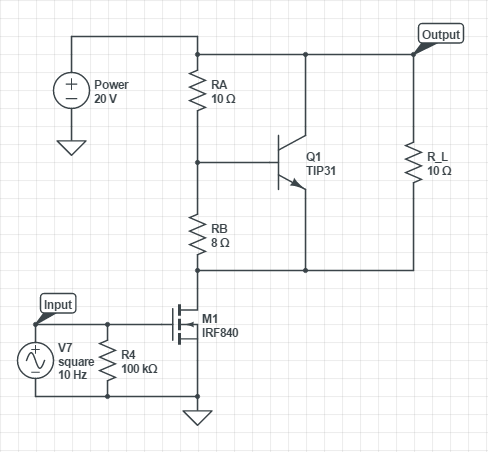
\includegraphics[scale=1]{img/figure_1}
		\caption{Final design of the shunt driver circuit}
		\label{fig_figure_1}
	\end{figure}S

\newpage

\begin{center}
\lstinputlisting{code_snips.c}
\end{center}

\eceSection{Results}

\eceSection{Conclusions}

\eceSection{Appendix}

\end{document} 

